\chapter[Desenvolvimento]{Desenvolvimento}
\label{cap:desenvolvimento}

Após o planejamento do projeto, foi feito o desenvolvimento de cada etapa.
Inicialmente, foi feito o desenvolvimento da placa de controle para poder acionar os motores.
Em seguida, o \textit{software} para o microcontrolador foi desenvolvido para realizar a leitura dos dados da manete e controlar o manipulador robótico.
Por último, foi desenvolvido o \textit{software} para o computador, que implementa a lógica do jogo de xadrez.

\section[Desenvolvimento da placa de controle]{Desenvolvimento da placa de controle}
\label{sec:desenvolvimentoPlacaControle}

Primeiramente, foi feito o desenvolvimento da placa de controle dos manipuladores, pois ela é necessária para as próximas etapas do projeto.
Para isso, foi necessário definir quais componentes utilizar e como conectá-los.

Conforme descrito na subseção \ref{sub:placaControle}, a placa de controle deve utilizar uma ponte H para o controle de cada junta.
Para isso, foi escolhido o CI L293D, que possui duas pontes H e suporta tensões de 12V.
Como é necessário controlar 6 motores, foram utilizados 3 CI L293D.

Para simplificar o controle e evitar problemas de acionamento duplo das entradas das pontes H, foi utilizado o CI 74LS02 como um inversor lógico.
Dessa forma, a placa de controle possui para cada junta uma entrada de \textit{Enable} para ligar/desligar o acionamento da junta, e uma porta de \textit{Direction} para definir a direção de movimentação dela.
A partir dessas entradas, o CI L293D é acionado e o motor é controlado.
A Figura \ref{fig:esquematicoSimplificado} mostra o esquemático simplificado de um CI L293D e um CI 74LS02.

\begin{figure}[H]
    \centering
    \caption{Esquemático simplificado de um CI L293D e um CI 74LS02}
    \includegraphics[keepaspectratio=true, width=0.9\textwidth]
    	{img/placa-controle-esquematico-simplificado.png}
    \fonte{Do próprio autor}
    \label{fig:esquematicoSimplificado}
\end{figure}

Com os componentes principais definidos foi feito o desenvolvimento do esquemático da placa de controle com o auxílio do software \textit{Altium Designer}.
O Apêndice \ref{apendice:esquematico-placa-controle} mostra o esquemático completo da placa de controle.
Nesse esquemático foram adicionados resistores de \textit{pulldown} para garantir que as entradas dos CI L293D e 74LS02 permaneçam em nível lógico baixo caso não estejam conectadas ao microcontrolador.
Também foram adicionadas \textit{LEDs} para indicar a alimentação de 5V e 12V da placa.

Após o desenvolvimento do esquemático, foi feita a montagem da Placa de Circuito Impresso (PCB), ainda com o auxílio do software \textit{Altium Designer}.
Para isso, os componentes foram posicionados no \textit{layout} da placa, tendo em vista a economia de espaço e a necessidade de manter os componentes próximos para facilitar sua conexão.
Em seguida, as trilhas e vias que realizam a conexão dos componentes foram desenhadas. 
Para permitir a conexão de todos os componentes, foi necessário utilizar uma placa com 2 camadas.
A Figura \ref{fig:placaControleLayout} mostra o \textit{layout} final da placa de controle.

Com o \textit{layout} finalizado, foi feita a produção da PCB de forma manual.
Para isso, o negativo do \textit{layout} foi impresso em uma folha de transparência.
Depois, uma placa de circuito impresso de duas camadas foi cortada no tamanho desejado.

Em seguida, foi feita a transferência do \textit{layout} para a placa.
Para isso, uma fina camada de tinta fotossensível destinada para PCB foi aplicada sobre a placa.
Essa tinta foi pré-curada à 75$^{\circ}$C durante 15 minutos com o auxílio de uma base de aquecimento, para garantir que ela não se descolasse da placa.
Após a pré-cura, a tinta foi exposta à luz ultravioleta por 3 minutos, utilizando a transparência com o \textit{layout} como máscara.
Em seguida, a placa foi submersa em uma solução de carbonato de sódio para realizar a revelação do \textit{layout}.
Após a placa ser revelada, a tinta foi curada à 85$^{\circ}$C durante 30 minutos.

Esse processo de transferência do \textit{layout} foi repetido para a segunda camada da placa.
Em seguida, foi utilizada uma solução de percloreto de ferro para corroer as áreas de cobre que não receberam tinta.
Após a corrosão, a placa foi mergulhada em uma solução de hidróxido de sódio para remover a tinta.

Após a corrosão da PCB, foi feita a perfuração das vias e dos furos para os componentes.
Por fim, foi feita a soldagem dos componentes na placa e a conexão das vias.
A Figura \ref{fig:placaControle} mostra a placa de controle montada.

\begin{figure}[H]
    \begin{minipage}{.5\textwidth}
        \centering
        \caption{Layout da placa de controle}
        \includegraphics[keepaspectratio=true, width=0.9\linewidth]
            {img/placa-controle-layout.png}
        \fonte{Do próprio autor}
        \label{fig:placaControleLayout}
    \end{minipage}%
    \begin{minipage}{.5\textwidth}
        \centering
        \caption{Placa de controle produzida}
        \includegraphics[keepaspectratio=true, width=0.9\linewidth]
            {img/placa-controle.jpg}
        \fonte{Do próprio autor}
        \label{fig:placaControle}
    \end{minipage}%    
\end{figure}

\section[Leitura da manete]{Leitura da manete}
\label{sec:leituraManete}

Após a montagem da placa de controle, foi iniciado o desenvolvimento do \textit{software} para o microcontrolador,
utilizando o \textit{software} \textit{PlatformIO}.

Inicialmente, foi implementada uma funcionalidade para realizar a leitura dos dados da manete que, 
conforme descrito na subseção \ref{sub:maneteJogador}, possui dois \textit{joysticks} com dois eixos e um botão cada.

Para realizar a leitura dos eixos dos \textit{joysticks}, foram utilizadas as entradas analógicas do microcontrolador.
Como o ESP32 utiliza um conversor analógico-digital de 12 bits, os valores lidos variam de 0 a 4095.
Valores próximos de 2048 representam a posição central do \textit{joystick}, enquanto valores próximos de 0 ou 4095 representam as posições extremas.
Para aprimorar a usabilidade da manete, foi implementada uma área de \textit{deadzone}, na qual o valor lido é considerado como zero,
para evitar que o manipulador se movimente sem a intenção do usuário.

Para realizar a leitura do botão, foi utilizada uma entrada digital.
Esses botões possuem um \textit{pull-up} interno, o que significa que o valor lido é 1 quando o botão não está pressionado e 0 quando o botão está pressionado.

Os valores lidos são armazenados em uma variável, que é utilizada por outras funcionalidades do \textit{software}.

\section[Leitura da posição das juntas]{Leitura da posição das juntas}
\label{sec:leituraPosicaoJuntas}

Para ler a posição das juntas do manipulador robótico, foi utilizado como base o \textit{software} desenvolvido anteriormente para ler os dados das manetes.

Primeiramente, foi utilizado um multímetro para medir o valor de tensão de saída do potenciômetro de cada junta em diferentes ângulos.
A partir disso, foi observado que a tensão de saída altera de forma aproximadamente linear com o ângulo,
e foi criada uma equação linear para cada junta, que relaciona a leitura realizada pelo microcontrolador com seu ângulo atual.

Com base nessas equações, foi implementada uma funcionalidade para calcular os valores que devem ser lidos pelo ESP32 quando o manipulador robótico estiver em uma determinada configuração.

\section[Controle dos motores]{Controle dos motores}
\label{sec:controleMotores}

O controle dos motores, responsável por mover o manipulador robótico para que ele atinja uma determinada configuração,
foi incorporado no software desenvolvido na seção anterior.

Para isso, foi implementado um controlador digital PID no microcontrolador ESP32.
Esse algoritmo realiza a leitura dos valores de tensão de cada junta e obtém o erro a partir da diferença entre o valor desejado e o valor atual.
A partir desse erro, é calculada a integral dos erros até o momento e a derivada entre o erro atual e o último erro.
Por fim, esses valores (erro atual, integral dos erros e derivada do erro) são multiplicados, respectivamente, por três constantes (Kp, Ki e Kd) e os resultados são somados.

Esse valor final é utilizado para definir os sinais de saída do microcontrolador para a placa de controle.
O módulo desse valor de saída do PID define o Duty Cycle do sinal de PWM, enquanto o seu sinal (positivo ou negativo) define a direção de movimentação do motor.

Depois da implementação do controlador PID foram feitos diversos testes para encontrar valores adequados para as constantes Kp, Ki e Kd.
Para isso, foi enviado um comando para movimentar uma junta para um determinado ângulo.
Após a junta estabilizar na posição desejada, foi enviado um outro comando para movimentá-la para um ângulo diferente, distante do primeiro.
Para alguns valores das constantes, foi observado um comportamento muito lento do sistema,
enquanto para outros valores foi observado um comportamento muito instável, com \textit{overshoot} e oscilações.
Depois de diversos testes, foram encontrados os valores apresentados na Tabela \ref{tab:constantesPID},
que possibilitam um movimento relativamente rápido e estável do manipulador robótico.

\begin{table}[H]
    \centering
    \caption{Constantes do controlador PID}
    \begin{tabular}{|c|c|c|c|}
        \hline
        \textbf{Junta} & \textbf{Kp} & \textbf{Ki} & \textbf{Kd} \\
        \hline
        Torso    & 400 & 10 & 5 \\
        \hline
        Ombro    & 500 & 40 & 0 \\
        \hline
        Cotovelo & 500 & 30 & 0 \\
        \hline
        Pulso    & 100 & 2 & 0.1 \\
        \hline        
    \end{tabular}
    \fonte{Do próprio autor}
    \label{tab:constantesPID}
\end{table}

\section[Cálculo dos ângulos desejados]{Cálculo dos ângulos desejados}
\label{sec:calculoAngulosDesejados}

Após implementar o controle do manipulador a  partir dos ângulos desejados para cada junta, foi necessário desenvolver o código que realiza o cálculo da configuração necessária para que o manipulador robótico alcance uma determinada posição no espaço.

Primeiramente, foi feita uma análise de como cada junta do manipulador robótico se movimenta.
Como pode ser observado na Figura \ref{fig:juntasManipulador},
o torso se movimenta horizontalmente, perpendicularmente ao eixo Z.
Por outro lado, o ombro, cotovelo e pulso se movimentam verticalmente, paralelamente à base do manipulador.

\begin{figure}[H]
    \centering
    \caption{Movimento das juntas do manipulador}
    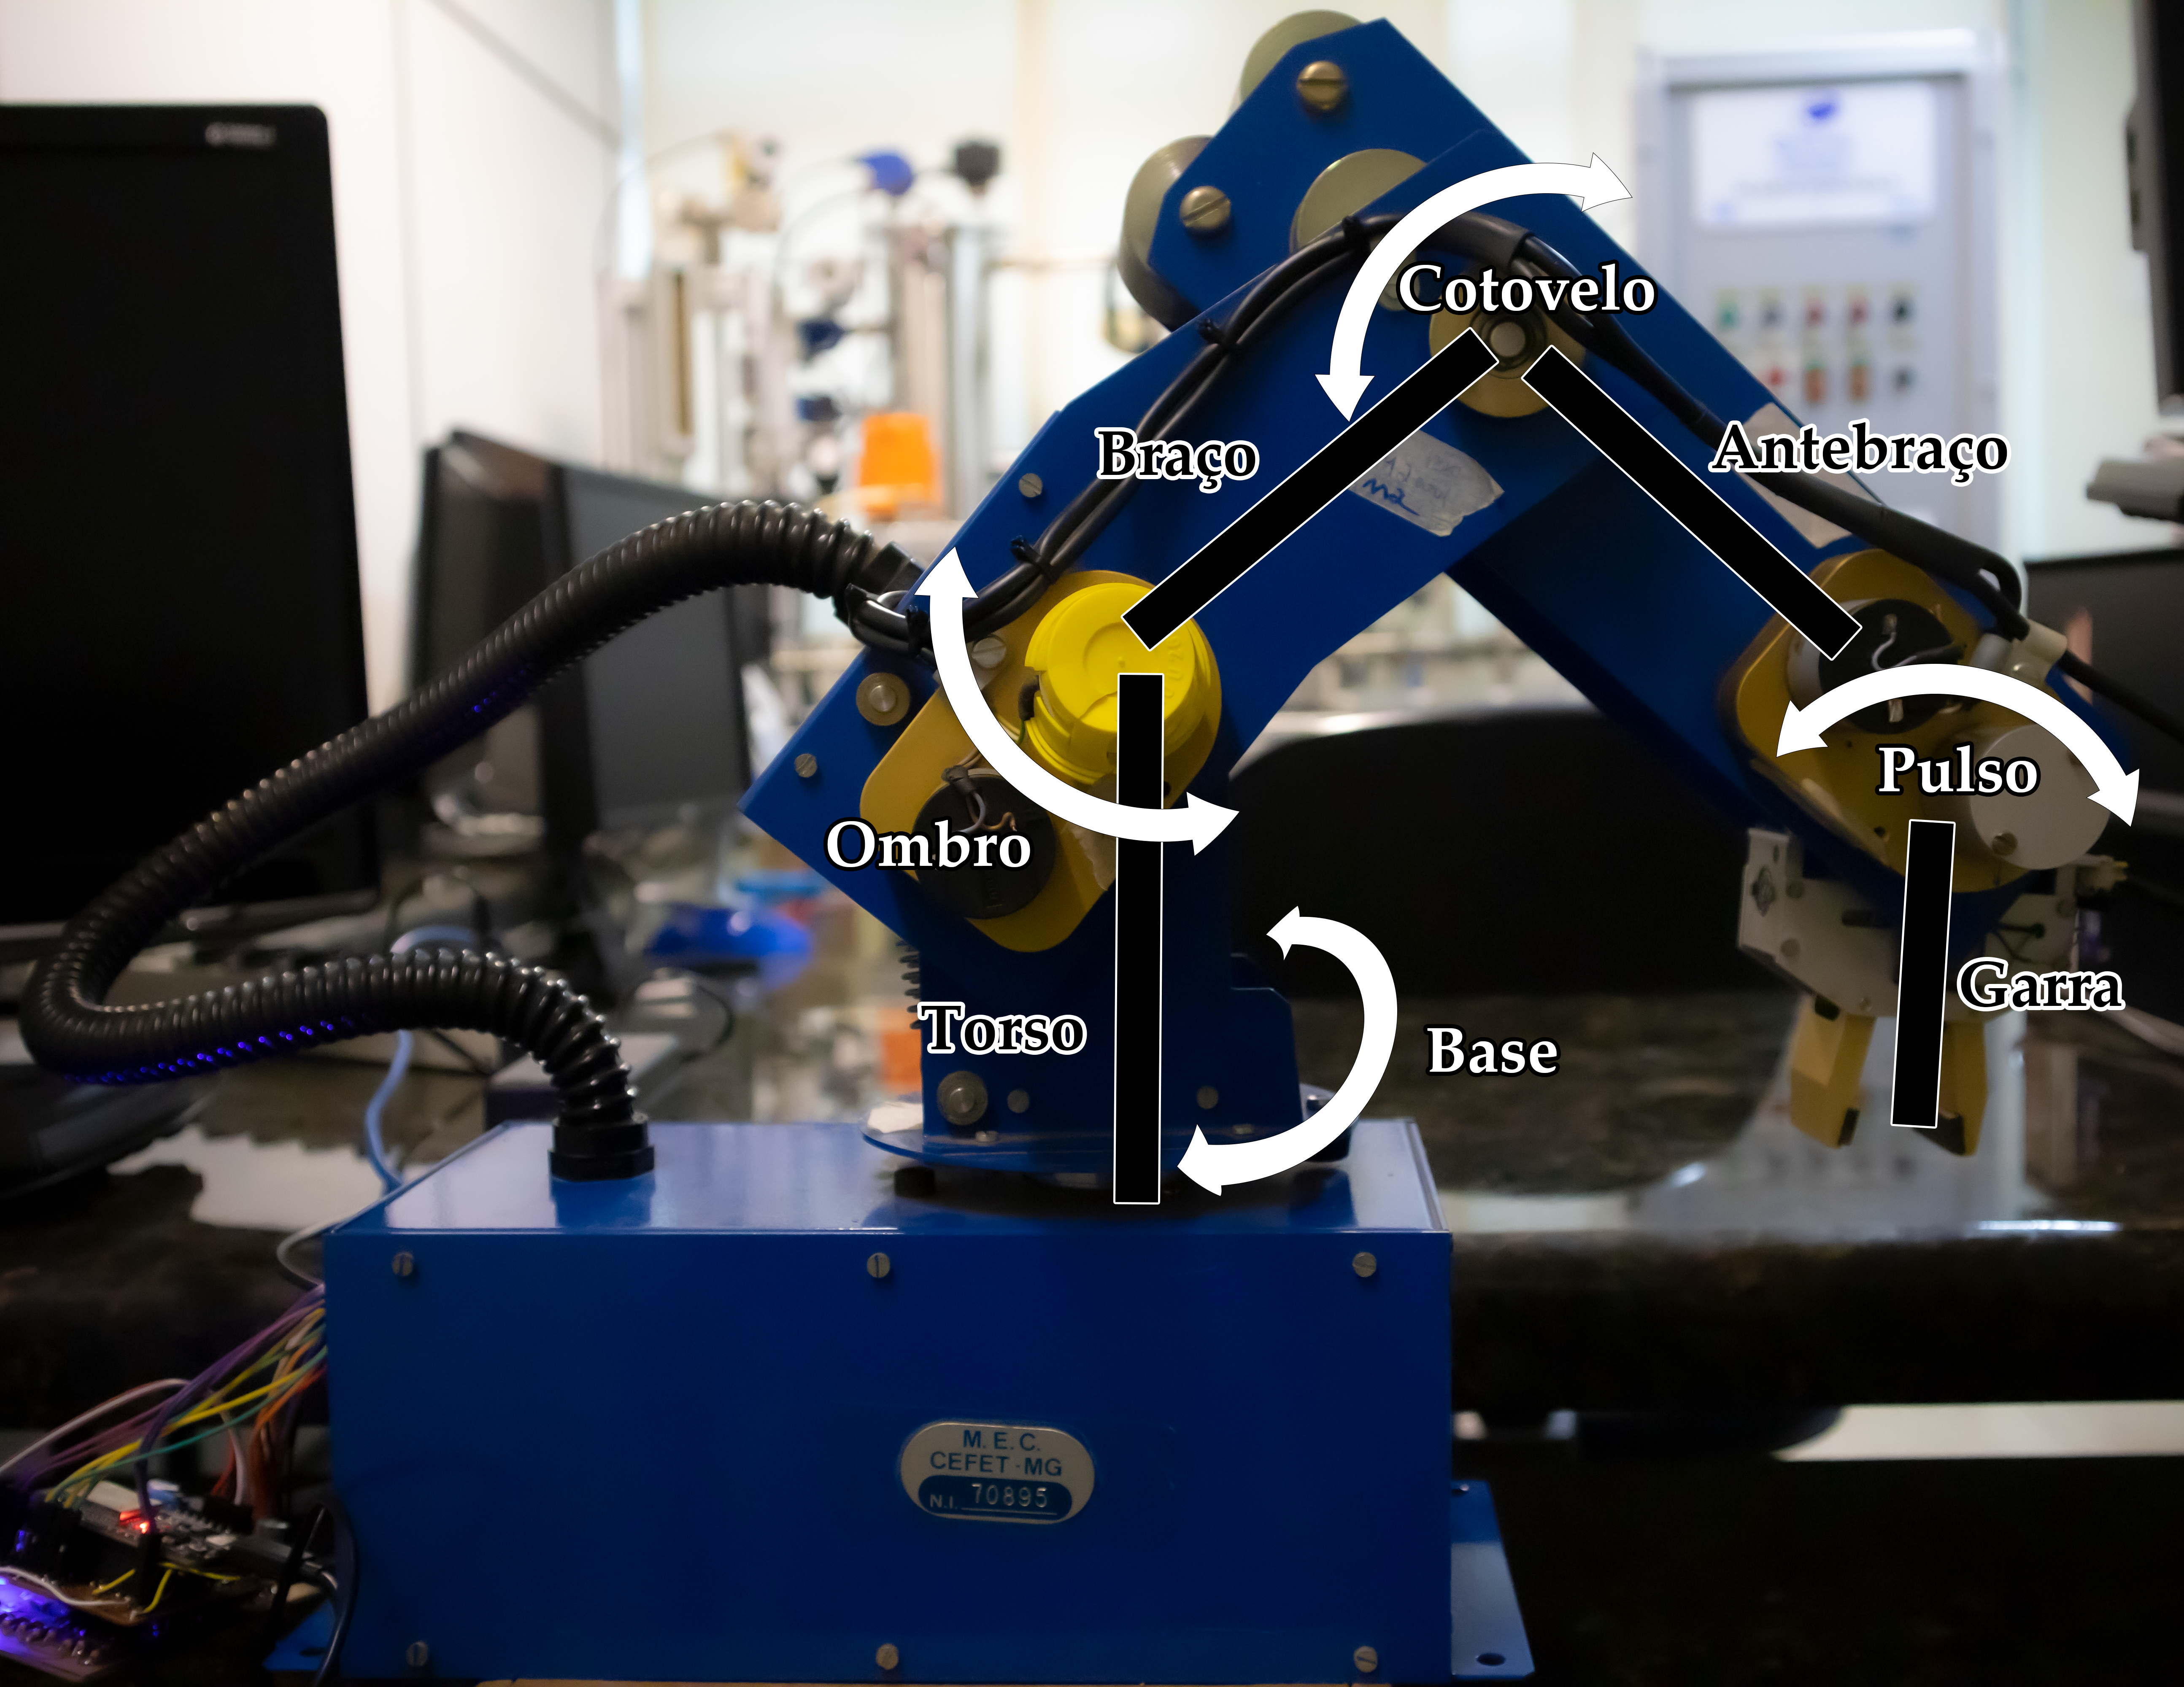
\includegraphics[keepaspectratio=true, width=1\textwidth]
    	{img/juntas-manipulador.png}
    \fonte{Do próprio autor}
    \label{fig:juntasManipulador}
\end{figure}

Em seguida, foi feita uma equação para o ângulo da primeira articulação (torso).
Como essa é a única junta capaz de rotacionar perpendicularmente ao eixo Z, seu ângulo pode ser calculado de forma independente das outras juntas, 
através apenas dos valores de x e y da posição desejada, ignorando o valor de z.
Como é possível observar na Figura \ref{fig:calculoAnguloTorso}, o ângulo dessa junta deve formar um triângulo retângulo com catetos de comprimento x e y.
A partir disso, o ângulo pode ser calculado como:

\begin{dmath}
\label{eq:anguloTorso}
    ânguloTorso = \arctan\left(\frac{x}{y}\right)
\end{dmath}

\begin{figure}[H]
    \centering
    \caption{Cálculo do ângulo do torso}
    \includegraphics[keepaspectratio=true, width=0.4\textwidth]
    	{img/Ângulo base.png}
    \fonte{Do próprio autor}
    \label{fig:calculoAnguloTorso}
\end{figure}

Em seguida, foi feito o cálculo dos ângulos restantes (ombro, cotovelo e pulso).
Para que seja possível pegar as peças sem interferir nas outras em casas próximas, é indispensável que a garra do manipulador esteja sempre perpendicular com o tabuleiro.
Dessa forma, apenas é necessário calcular os ângulos das duas juntas restantes de forma que o ombro termine nas posições x e y desejadas e a uma altura igual ao z desejado mais o comprimento da garra.

Com base nisso, podemos simplificar os dados necessários para calcular os ângulos do ombro e do cotovelo.
Essa parte do manipulador deve ter um comprimento total definido pela hipotenusa do triângulo retângulo apresentado na Figura \ref{fig:calculoAnguloTorso}, com catetos x e y.
E sua altura total deve ser igual ao z desejado, subtraído dos comprimentos da garra e do torso do manipulador. Portanto, temos as seguintes equações:

\begin{dmath}
\label{eq:comprimentoOmbroCotovelo}
    comprimento = \sqrt{x^2 + y^2}
\end{dmath}

\begin{dmath}
\label{eq:alturaOmbroCotovelo}
    altura = z - comprimentoTorso - comprimentoGarra
\end{dmath}

A partir desses valores de comprimento e altura, o cálculo desses ângulos se reduz a um problema de cinemática inversa de um manipulador com dois graus de liberdade.
Existem duas soluções para esse tipo de problema, uma com o ângulo do segundo eixo positivo em relação ao primeiro, e outra com esse ângulo negativo.
Devido às limitações da movimentação do ombro do manipulador utilizado, foi escolhida a solução na qual o ângulo do cotovelo é negativo, descrita pelas equações abaixo. \cite{inverse_kinematics}

\begin{dmath}
\label{eq:anguloCotovelo}
    ânguloCotovelo = -\arccos\left(\frac{comprimento^2 + altura^2 - comprimentoBraço^2 - comprimentoAntebraço^2}{2 \cdot comprimentoBraço \cdot comprimentoAntebraço}\right)
\end{dmath}

\begin{dmath}
\label{eq:anguloCotovelo}
    ânguloOmbro = \arctan{\frac{altura}{comprimento}} + \arcsin\left(\frac{comprimentoAntebraço \cdot \sin\left(ânguloCotovelo\right)}{comprimentoBraço + comprimentoAntebraço \cdot \cos\left(ânguloCotovelo\right)}\right)
\end{dmath}

Por último, resta calcular o ângulo do pulso, que deve ficar perpendicular ao tabuleiro.
Para isso, pode ser descrito um quadrilátero envolvendo o braço, antebraço, pulso e o tabuleiro, conforme representado na Figura \ref{fig:calculoAnguloPulso}.
Como a soma dos ângulos internos de um quadrilátero deve ser igual a 360$^{\circ}$, pode-se obter a equação abaixo:

\begin{dmath}
\label{eq:anguloPulso}
        ânguloPulso = 90 - ânguloOmbro - ânguloCotovelo
\end{dmath}

\begin{figure}[H]
    \centering
    \caption{Cálculo do ângulo do pulso}
    \includegraphics[keepaspectratio=true, width=0.4\textwidth]
    	{img/Ângulo Pulso.png}
    \fonte{Do próprio autor}
    \label{fig:calculoAnguloPulso}
\end{figure}

Para facilitar a visualização dos ângulos e permitir uma comparação visual entre a posição desejada do manipulador e sua posição real,
foi desenvolvido um simples \textit{script} em Python que implementa um modelo simplificado do manipulador.
Esse \textit{script} permite movimentar o modelo para uma determinada posição x, y e z, e exibe os ângulos calculados para cada junta.
A Figura \ref{fig:modeloManipulador} mostra o modelo desenvolvido.

\begin{figure}[H]
    \centering
    \caption{Modelo simplificado do manipulador}
    \includegraphics[keepaspectratio=true, width=1\textwidth]
    	{img/modelo-manipulador.png}
    \fonte{Do próprio autor}
    \label{fig:modeloManipulador}
\end{figure}

\section[Movimentação de peças]{Movimentação de peças}
\label{sec:movimentacaoPecas}

Depois de desenvolvida a funcionalidade de cálculo dos ângulos para movimentar o manipulador para uma determinada posição, foi necessário adicionar uma funcionalidade para utilizar o manipulador para pegar, mover e soltar as peças de xadrez.

Para isso, foi primeiramente definido de forma prática uma altura de movimentação do manipulador, que permite que ele mova livremente sem derrubar nenhuma peça e 
uma altura para pegar as peças, na qual a garra consegue alcançar e pegar qualquer peça.
Em seguida, foram mapeadas as coordenadas x e y de todas as casas do tabuleiro. Devido à uma limitação no tamanho do manipulador utilizado, não foi possível alcançar algumas casas, portanto as peças nessas casas devem ser movimentadas manualmente pelo jogador.

A partir disso, foi implementada uma funcionalidade para movimentar o manipulador para uma determinada casa do tabuleiro, apenas nos eixos x e y.
Em seguida, foi adicionada uma funcionalidade para pegar e outra para soltar a peça que está na casa atual do manipulador, movimentando-o apenas no eixo z e acionando a garra.
Por fim, foi feita uma funcionalidade para movimentar o manipulador para a posição de repouso e outra para movimentá-lo para a posição de descarte de peças.

Devido à relação não linear entre os ângulos das juntas e a posição do manipulador,
foi observado que o manipulador não se movimentava adequadamente entre as casas do tabuleiro,
frequentemente derrubando peças.
Para solucionar esse problema, cada movimento do manipulador foi dividido em diversos movimentos menores,
de forma que o manipulador se movimente de forma mais suave e controlada.

\section[Comunicação com o computador]{Comunicação com o computador}
\label{sec:comunicacaoComputador}

Após finalizar a movimentação das peças, foi desenvolvido o módulo responsável por realizar a comunicação entre o microcontrolador e o computador.

Conforme descrito na subseção \ref{sub:computador}, essa comunicação é feita através do protocolo serial, por meio de um cabo USB.
Entretanto, ainda era necessário definir o formato dos dados que serão enviados e recebidos.

Para isso, foram definidos alguns comandos que podem ser enviados pelo computador para o microcontrolador, conforme descrito na Tabela \ref{tab:comandosMicrocontrolador}.

\begin{table}[H]
    \centering
    \caption{Comandos enviados pelo computador para o microcontrolador}
    \begin{tabular}{|c|c|c|}
        \hline
        \textbf{Comando} & \textbf{Descrição} & \textbf{Formato} \\
        \hline
        move & Movimentar para casa & move x y \\
        \hline
        grab & Pegar peça & grab \\
        \hline
        release & Soltar peça & release \\
        \hline
        discard & Movimentar para posição de descarte & discard \\
        \hline
        reset & Movimentar para posição de repouso & reset \\
        \hline
        wait & Aguarde por x milisegundos & wait x \\
        \hline
    \end{tabular}
    \fonte{Do próprio autor}
    \label{tab:comandosMicrocontrolador}
\end{table}

Ao final da execução de cada comando, o microcontrolador envia uma mensagem de confirmação para o computador, informando se o comando foi executado com sucesso (OK) ou não (FAIL).

Para possibilitar o controle manual do manipulador, foram definidas algumas mensagens que podem ser enviadas pelo microcontrolador para o computador, conforme descrito na Tabela \ref{tab:mensagensMicrocontrolador}.

\begin{table}[H]
    \centering
    \caption{Mensagens enviadas pelo microcontrolador para o computador}
    \begin{tabular}{|c|c|c|}
        \hline
        \textbf{Mensagem} & \textbf{Descrição} & \textbf{Formato} \\
        \hline
        joystick & \textit{Joystick} foi movimentado & joystick <up down left right> \\
        \hline
        select & Botão do \textit{joystick} foi pressionado & select \\
        \hline
    \end{tabular}
    \fonte{Do próprio autor}
    \label{tab:mensagensMicrocontrolador}
\end{table}

\section[Implementação da lógica de xadrez]{Implementação da lógica de xadrez}
\label{sec:implementacaoLogicaXadrez}

Depois de finalizar a comunicação entre o microcontrolador e o computador, foi desenvolvido o \textit{software} responsável por implementar a lógica do jogo de xadrez.

O \textit{software} foi desenvolvido em Python, utilizando a biblioteca stockfish \cite{stockfish_python} para realizar comunicação com a \textit{engine} de xadrez Stockfish 15.1 \cite{stockfish_engine}.
Essa \textit{engine} é responsável por verificar quais movimentos são válidos e calcular qual movimento o computador deve jogar em cada turno.

Além da utilização da biblioteca stockfish, foi necessário implementar algumas funcionalidades manualmente que não existem nela.
Em primeiro lugar, foi implementada uma função para adquirir quais movimentos são válidos para a posição atual do tabuleiro, utilizando o comando \textit{go perft 1} da \textit{engine} Stockfish.
Em seguida, foi desenvolvida uma funcionalidade para detectar quando a partida acabou, verificando se não existe mais nenhum movimento válido para o jogador atual.
Por último, foi feita uma função para verificar se o jogo terminou empatado, verificando a avaliação da posição atual do tabuleiro pela \textit{engine} Stockfish.

Para comunicar com o microcontrolador, foi utilizada a biblioteca PySerial \cite{pyserial}.
Através dessa biblioteca, é possível enviar e receber as mensagens descritas na seção \ref{sec:comunicacaoComputador}.
Após enviar uma mensagem para o microcontrolador, o \textit{software} aguarda uma mensagem de confirmação para indicar o sucesso ou falha da execução do comando.

O programa desenvolvido suporta dois modos de jogo: jogar contra o computador ou contra outra pessoa.
No primeiro modo, o \textit{software} Stockfish 15.1 é utilizado para calcular qual movimento o computador irá jogar, 
enquanto no segundo modo, o jogador que estiver controlando o manipulador pode movimentá-lo pelas casas do tabuleiro e pegar peças sem restrição, entretanto ao tentar soltar uma peça, é feita uma consulta ao Stockfish 15.1 para validar se a jogada desejada é válida.
Em ambos os modos de jogo, os movimentos realizados pelo jogador humano que não controla o manipulador robótico devem ser digitados manualmente no computador.

Ao detectar uma captura de peça, o programa primeiro controla o manipulador para movimentar a peça capturada para a posição de descarte.
Em seguida é feita a movimentação da peça que capturou para a casa de destino.
Foi feito um tratamento especial para capturas do tipo \textit{en passant}, pois nesses movimentos a peça capturada não está na casa de destino.

Um outro tratamento especial foi feito para movimentos de roque, pois nesses movimentos duas peças são movimentadas ao mesmo tempo.

Por fim, caso o manipulador robótico esteja jogando com as peças pretas,
o programa realiza uma conversão da posição do tabuleiro para realizar o movimento adequado.